% Made up for the tikra benchmark.
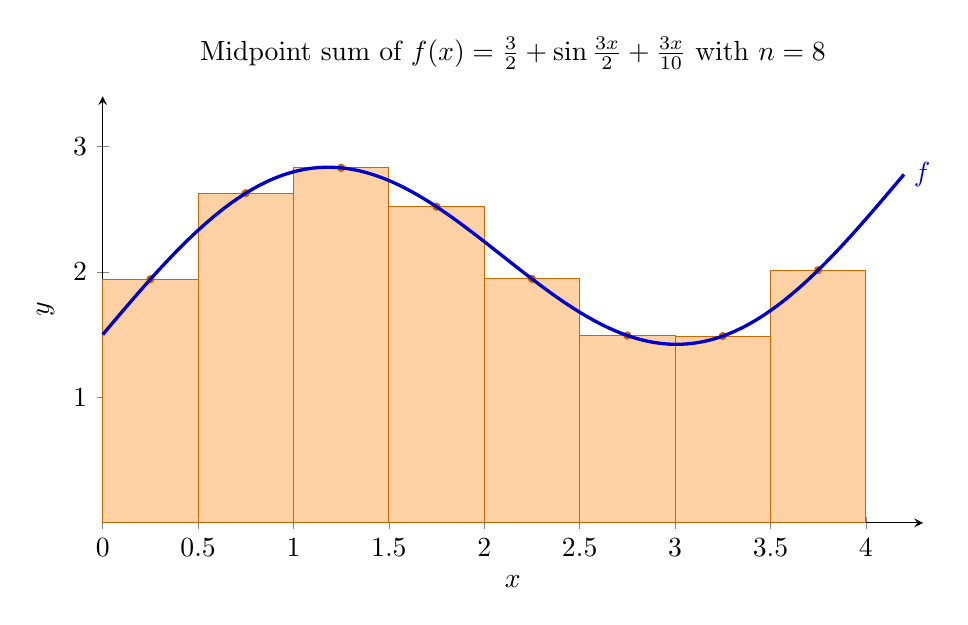
\begin{tikzpicture}[declare function={f(\x) = 1.5 + sin(deg(1.5*\x)) + 0.3*\x;}]
\begin{axis}[width=12cm, height=7cm, axis lines=left, xmin=0, xmax=4.3, ymin=0, ymax=3.4,
    xlabel=$x$, ylabel=$y$, xtick={0,0.5,...,4}, ytick={1,2,3}, clip=false,
    title={Midpoint sum of $f(x) = \frac32 + \sin\frac{3x}{2} + \frac{3x}{10}$ with $n = 8$}]
  \pgfplotsinvokeforeach{0,0.5,...,3.5}{
    \draw[fill=orange!35, draw=orange!80!black] (axis cs:#1,0) rectangle (axis cs:#1+0.5,{f(#1+0.25)});
    \fill[orange!80!black] (axis cs:#1+0.25,{f(#1+0.25)}) circle (1.5pt);
  }
  \addplot[very thick, blue!80!black, domain=0:4.2, samples=120] {f(x)};
  \node[blue!80!black, anchor=west] at (axis cs:4.2,{f(4.2)}) {$f$};
\end{axis}
\end{tikzpicture}
